\documentclass{article}\usepackage[]{graphicx}\usepackage[]{xcolor}
% maxwidth is the original width if it is less than linewidth
% otherwise use linewidth (to make sure the graphics do not exceed the margin)
\makeatletter
\def\maxwidth{ %
  \ifdim\Gin@nat@width>\linewidth
    \linewidth
  \else
    \Gin@nat@width
  \fi
}
\makeatother

\definecolor{fgcolor}{rgb}{0.345, 0.345, 0.345}
\newcommand{\hlnum}[1]{\textcolor[rgb]{0.686,0.059,0.569}{#1}}%
\newcommand{\hlstr}[1]{\textcolor[rgb]{0.192,0.494,0.8}{#1}}%
\newcommand{\hlcom}[1]{\textcolor[rgb]{0.678,0.584,0.686}{\textit{#1}}}%
\newcommand{\hlopt}[1]{\textcolor[rgb]{0,0,0}{#1}}%
\newcommand{\hlstd}[1]{\textcolor[rgb]{0.345,0.345,0.345}{#1}}%
\newcommand{\hlkwa}[1]{\textcolor[rgb]{0.161,0.373,0.58}{\textbf{#1}}}%
\newcommand{\hlkwb}[1]{\textcolor[rgb]{0.69,0.353,0.396}{#1}}%
\newcommand{\hlkwc}[1]{\textcolor[rgb]{0.333,0.667,0.333}{#1}}%
\newcommand{\hlkwd}[1]{\textcolor[rgb]{0.737,0.353,0.396}{\textbf{#1}}}%
\let\hlipl\hlkwb

\usepackage{framed}
\makeatletter
\newenvironment{kframe}{%
 \def\at@end@of@kframe{}%
 \ifinner\ifhmode%
  \def\at@end@of@kframe{\end{minipage}}%
  \begin{minipage}{\columnwidth}%
 \fi\fi%
 \def\FrameCommand##1{\hskip\@totalleftmargin \hskip-\fboxsep
 \colorbox{shadecolor}{##1}\hskip-\fboxsep
     % There is no \\@totalrightmargin, so:
     \hskip-\linewidth \hskip-\@totalleftmargin \hskip\columnwidth}%
 \MakeFramed {\advance\hsize-\width
   \@totalleftmargin\z@ \linewidth\hsize
   \@setminipage}}%
 {\par\unskip\endMakeFramed%
 \at@end@of@kframe}
\makeatother

\definecolor{shadecolor}{rgb}{.97, .97, .97}
\definecolor{messagecolor}{rgb}{0, 0, 0}
\definecolor{warningcolor}{rgb}{1, 0, 1}
\definecolor{errorcolor}{rgb}{1, 0, 0}
\newenvironment{knitrout}{}{} % an empty environment to be redefined in TeX

\usepackage{alltt}
\title{\textbf{R Homework Two}}
\author{\textbf{Katherine Wolf}\\ Introduction to Causal Inference (PH252D)\\ \today}
\date{}

% list of latex packages you'll need
\usepackage{float}  % for tables
\usepackage{mathtools}  % for mathematical symbols
\usepackage{bm}  % to bold mathematical symbols like betas
\usepackage{scrextend}  % to indent subsections
\usepackage{xltxtra}
\usepackage{fontspec}
\usepackage{xunicode}
\usepackage[skip=0.5\baselineskip]{caption}  % control caption printing space
\usepackage{longtable}
\usepackage{amsmath}
\usepackage{amsfonts}
\usepackage{bm}
\usepackage{caption}
\usepackage[shortlabels]{enumitem}
\usepackage{txfonts}
\usepackage{dejavu}
\usepackage{mathpazo}

% set fonts
\setmainfont{Palatino Linotype}
\setsansfont{Corbel}
\setmonofont{Consolas}

% make special code formatting
\NewDocumentCommand{\codeword}{v}{%
  \texttt{{#1}}%
}

% set the margins of the document
\usepackage[top=1in, bottom=1in, left=.5in, right=.5in]{geometry}



% end the preamble and begin the document
\IfFileExists{upquote.sty}{\usepackage{upquote}}{}
\begin{document}

\maketitle

\section{Time to prevent child malnutrition in Sahel}

\section{A specific data generating process}

  \subsection{Evaluate the positivity assumption in closed form for this data generating process.}
  
  \subsection{Evaluate the statistical estimand $\Psi(\mathbb{P}_O)$ in closed form for this data generating process.}
  
\section{Translate this data generating process into simulations}

  \subsection{First set the seed to 252.}
  
  \subsection{Set the number of draws $n = 100,000$.}
  
  \subsection{Sample $n$ independent and identically distributed (i.i.d.) observations of random variable $O=(W1,W2,A,Y) \sim \mathbb{P}_O$.}
  
  \subsection{\textit{Bonus}: Intervene to set the exposure to the combination package $(A=1)$ and generate the counterfactual outcome $Y_1$. Intervene to set the exposure to the standard of care $(A=0)$ and generate the counterfactual outcomes $Y_0$. Evaluate the causal parameter $\Psi^F(\mathbb{P}_{U,X})$.}
  
  \subsection{Evaluate the positivity assumption.}
  
  \subsection{Evaluate the statistical estimand $\Psi(\mathbb{P}_O)$ and assign the value $\psi_0$ to \texttt{Psi.P0}.}
  
  \subsection{Interpret $\Psi(\mathbb{P}_O)$.}
  
\section{The simple substitution estimator based on the G-compuation formula}

  \subsection{Set the number of iterations $R$ to 500 and the number of observations $n$ to 200. Do not reset the seed.}
  
  \subsection{Create a $R = 500$ by 4 matrix \texttt{estimates} to hold the resulting estimates obtained at each iteration.}
  
  \subsection{Inside a \texttt{for} loop from $r = 1$ to $r = R = 500$, do the following.}
  
  \begin{enumerate}[label=\textbf{\alph*.}]
  
    \item Sample $n$ i.i.d. observations of $O = (W1,W2,A,Y)$.
    
    \item Create a data frame \texttt{obs} of the resulting observed data.
    
    \item Copy the dataset \texttt{obs} into two new data frames \texttt{txt} and \texttt{control}. Then set \texttt{A=1} for all units in \texttt{txt} and set \texttt{A=0} for all units in \texttt{control}.
    
    \item Estimator 1: Use \texttt{glm} function to estimate $\bar{Q}_0(A,W)$ (the conditional probability of survival, given the intervention and baseline covariates) based on the following parametric regression model:
    
\begin{align*}
\bar{Q}^1_0(A,W)=logit^{-1}(\beta_0+\beta_1A)
\end{align*}

Be sure to specify the arguments \texttt{family='binomial'} and \texttt{data=obs}.

    \item Estimator 2: Use Use \texttt{glm} function to estimate $\bar{Q}_0(A,W)$ based on the following parametric regression model:
    
\begin{align*}
\bar{Q}^2_0(A,W)=logit^{-1}(\beta_0+\beta_1A+\beta_2W1)
\end{align*}

Be sure to specify the arguments \texttt{family='binomial'} and \texttt{data=obs}.

    \item Estimator 3: Use \texttt{glm} function to estimate $\bar{Q}_0(A,W)$ (the conditional probability of survival, given the intervention and baseline covariates) based on the following parametric regression model:
    
\begin{align*}
\bar{Q}^3_0(A,W)=logit^{-1}(\beta_0+\beta_1A+\beta_2W2)
\end{align*}

Be sure to specify the arguments \texttt{family='binomial'} and \texttt{data=obs}.
    
    \item Estimator 4: Use \texttt{glm} function to estimate $\bar{Q}_0(A,W)$ (the conditional probability of survival, given the intervention and baseline covariates) based on the following parametric regression model:
    
\begin{align*}
\bar{Q}^4_0(A,W)=logit^{-1}(\beta_0+\beta_1A+\beta_2W1+\beta_3W2+\beta_4A*W1+\beta_5A*W2)
\end{align*}

Be sure to specify the arguments \texttt{family='binomial'} and \texttt{data=obs}.
    
    \item For \textit{each} estimator of $\bar{Q}_0(A,W)$, use the \texttt{predict} function to get the expected (mean) outcome for each unit under the intervention $\bar{Q}_n(1,W_i)$. Be sure to specify the arguments \texttt{newdata=control} and \texttt{type='response'}.
    
    \item For \textit{each} estimator of $\bar{Q}_0(A,W)$, use the \texttt{predict} function to get the expected (mean) outcome for each unit under the intervention $\bar{Q}_n(0,W_i)$. Be sure to specify the arguments \texttt{newdata=control} and \texttt{type='response'}.
    
    \item For \textit{each} estimator of $\bar{Q}_0(A,W)$, estimate $\Psi(\mathbb{P}_0)$ by substituting the predicted mean outcomes under the treatment $\bar{Q}_n(1,W_i)$ and control $\bar{Q}_n(0,W_i)$ into the G-computation formula and using the sample proportion to estimate the marginal distribution of baseline covariates:
    
\begin{align*}
\hat{\Psi(\mathbb{n})}=\frac{1}{n}\sum{i=1}{n}[\bar{Q}_n(1,W_i)-\bar{Q}_n(0,W_i)]
\end{align*}
    
    \item Assign the resulting values as a row in matrix \texttt{estimates}.
    
  \end{enumerate}
    
\section{Performance of the estimators}

  \subsection{What is the average value of each estimator of $\Psi(\mathbb{P}_0)$ across $R=500$ simulations?}
  
  \subsection{Estimate the bias of each estimator.}
  
  \subsection{Estimate the variance of each estimator.}
  
  \subsection{Estimate the mean squared error (MSE) of each estimator.}

  \subsection{Briefly comment on the performance of the estimators. Which estimator has he lowest MSE over the $R=500$ iterations? Are you surprised?}
 
 
 
 
 
 
 
 
 
 
 
 
 
 
 
 
 
 
 
 
 
 
 
 
 
 
 
 
    
\begin{knitrout}
\definecolor{shadecolor}{rgb}{0.969, 0.969, 0.969}\color{fgcolor}
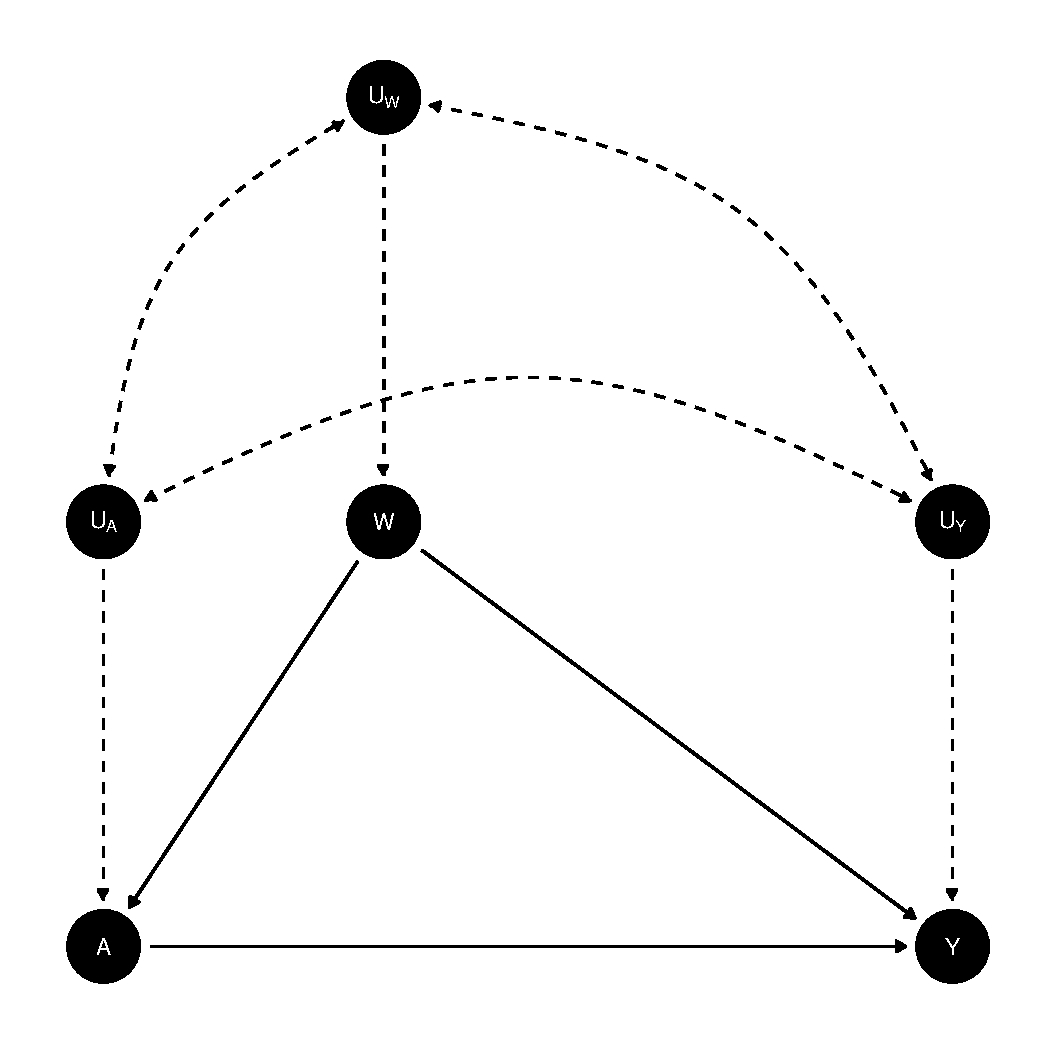
\includegraphics[width=4in]{figure/unnamed-chunk-2-1} 

\end{knitrout}
      
      
      
\end{document}
